\begin{figure*}[t]
\centering
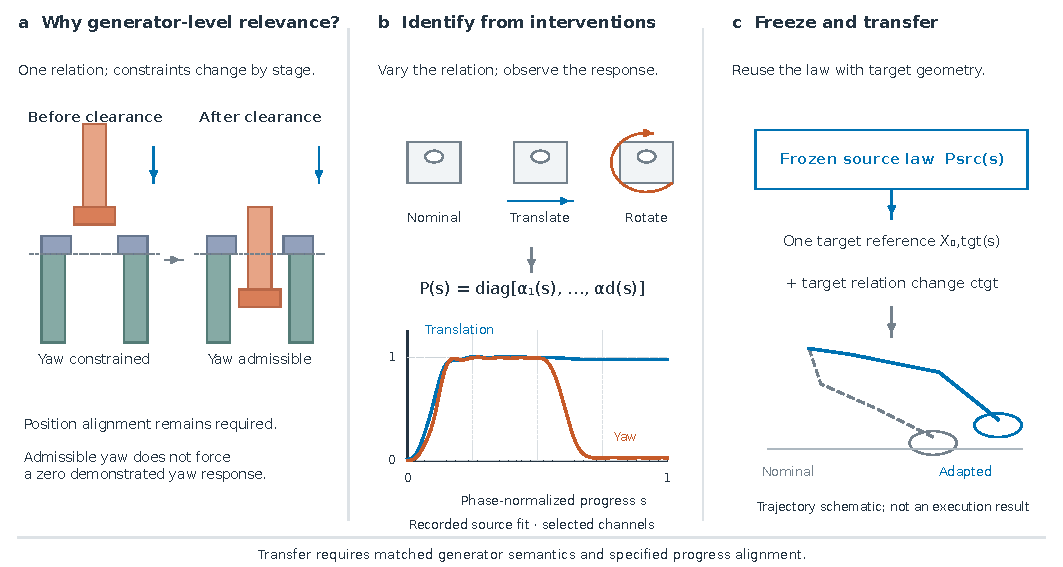
\includegraphics[width=\textwidth]{fig1_method.pdf}
\caption{Generator-level response identification and matched-relation transfer. (a) Schematic keyed insertion illustrates how admissible motion changes after key clearance while positional alignment remains required. Geometric permission does not uniquely determine the demonstrated response. (b) Controlled relation interventions provide supervision for a generator-wise model. The inset reproduces selected translation and yaw outputs of an archived finite diagonal source fit; it illustrates the representation, not cross-strategy invariance or an uncertainty estimate. (c) The frozen source model is combined with one target nominal trajectory and the target relation change. The paths are schematic, not measured hardware results. Transfer is evaluated under matched generator semantics and specified progress alignment.}
\label{fig:method_overview}
\end{figure*}
